\chapter{Negative friction coefficient}\label{chap:negative_coef}

For the final part of this thesis, we concern ourselves with a proof of concept approach for the designing of a negative friction coefficient. From the pilot study (\cref{chap:pilot_study}) we found the two investigated patterns to have a non-linear relationship with strain which is hypothesized to yield a negative friction coefficeint in a coupled system system of load and strain for certain load ranges. We will investigate this hypothesis further in this chapter.

\section{Nanomachine coupling}
We do not attempt to simulate the dynamics of any nanomachine desings, but we propose that a coupling could be achieved, for instance by following a design as sketched in \cref{fig:nanomachine}. Such a design could perhaps be achieved by rigging carbon nanotubes in a similar configuration. 

\begin{figure}[H]
  \centering
  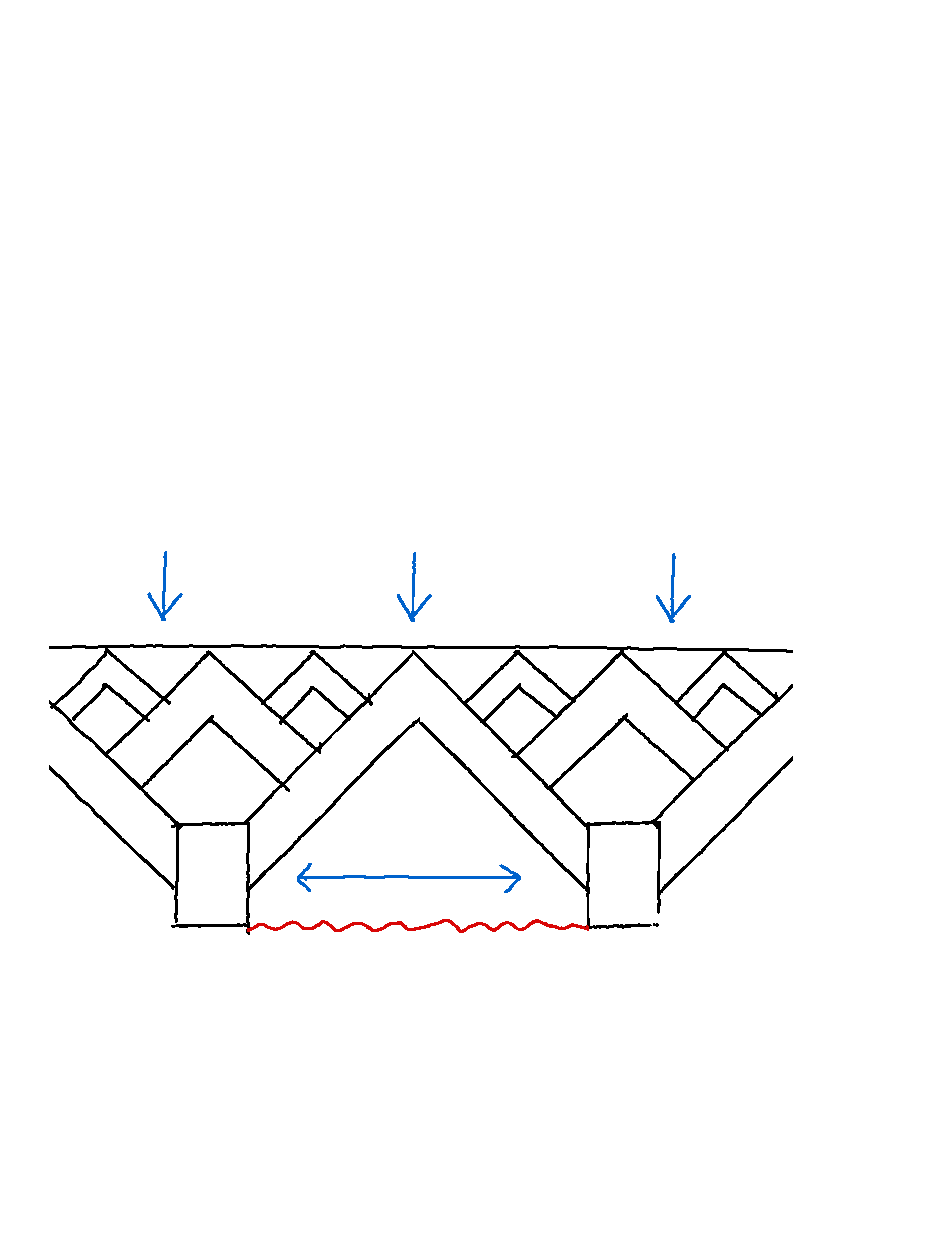
\includegraphics[width=0.5\linewidth]{figures/negative_coefficient/nanomachine.pdf}
  \caption{Working sketch for nanomachine}
  \label{fig:nanomachine}
\end{figure}

We mimic the nanomachine coupling by implementing a load-depending tension force to our \acrshort{MD} simulations. So far, we have kept the pull block spaced by a fixed distance throuhout the simulations, but now we let the pull blocks move relative to each other under the influence of this tenstion force between the blocks. The tension force $F_t$ is modeled to be linearly coupled to normal load $F_t = TF_N$ by a factor $T$ which represents the ratio for the load to strain coupling. We find that a ratio of
$T=6$ will provide the necessary tension for achieving a full strain range (till rupture) within the loading range used so far in our study. Notice that this coupling scheme is slightly different than that proposed in~\cref{eq:mu_strain} where we assumed a coupling between load and strain $\varepsilon = R F_N$. This is done to provide a standardized description of the proposed nanomachine for which the relation between tension and strain will depend on the specific Kirigami sheet. We use the Tetrahedron
$(7,5,1)$ and Honeycomb $(2,2,1,5)$ from the pilot study and perform multiple
simulations for different loads. We sample 100 pseudo uniform normal force
values in the $[0, 15]$ nN which corresponds to a tension force of $[0, 90]$ nN. For the Tetrahedron pattern we increase the load by a speed of \SI{0.015}{nN/ps}. Due to a rapid change in the strain-tension curve for the Honeycomb pattern we reduced the loading speed to \SI{0.0015}{nN/ps} and added additional data points to the sparsely populated strain range. By considering the strain-load curve we map compare the results from the pilot study \cref{fig:multi_stretch} by mapping the strain values to the corresponding load values of our coupled system. The results are shown in \cref{fig:negfric}.


\begin{figure}[H]
  \centering
  \begin{subfigure}[t]{\textwidth}
      \centering
      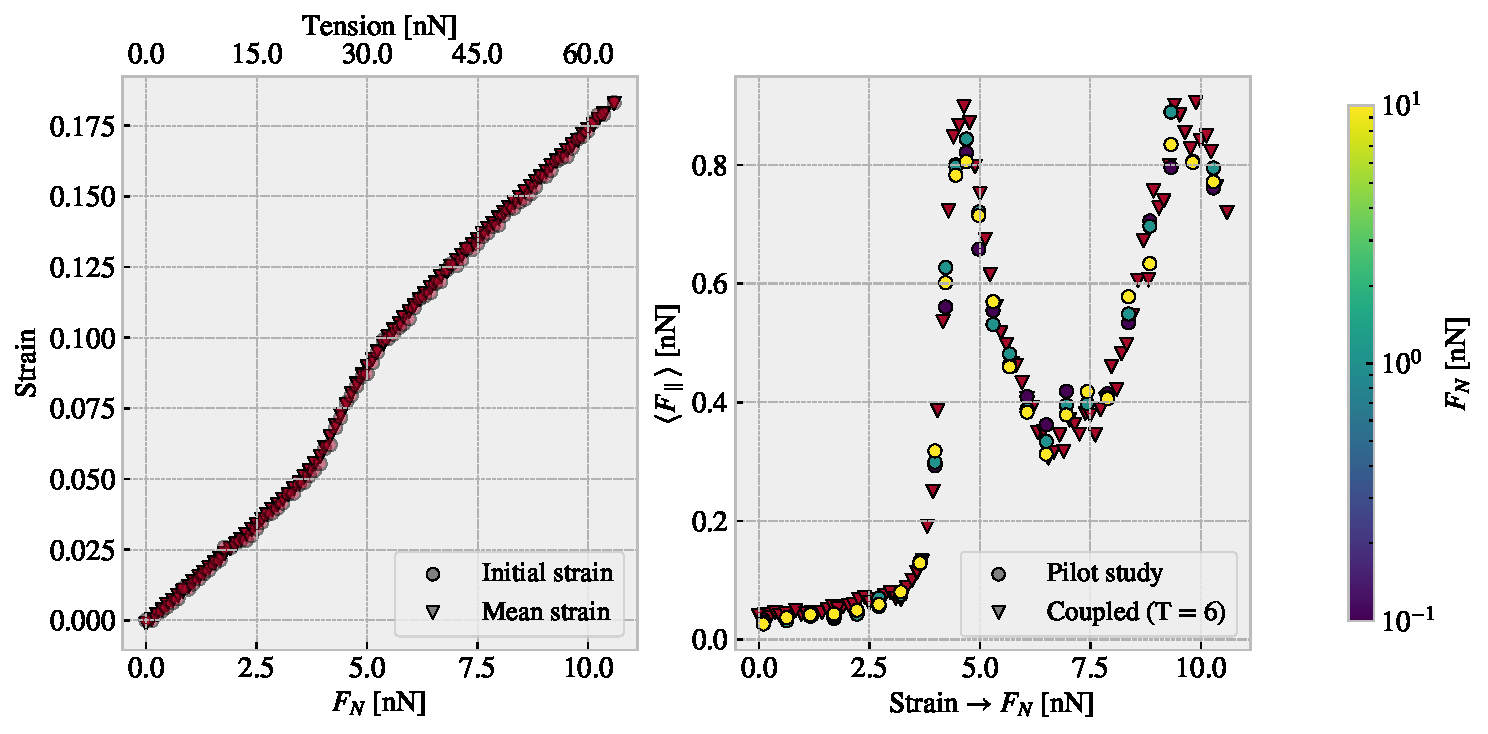
\includegraphics[width=\textwidth]{figures/negative_coefficient/manual_coupling_tension_pop7_5_1.pdf}
      \caption{Tetrahedron $(7,5,1)$}
      % \label{fig:}
  \end{subfigure}
  \hfill
  \begin{subfigure}[t]{\textwidth}
    \centering
    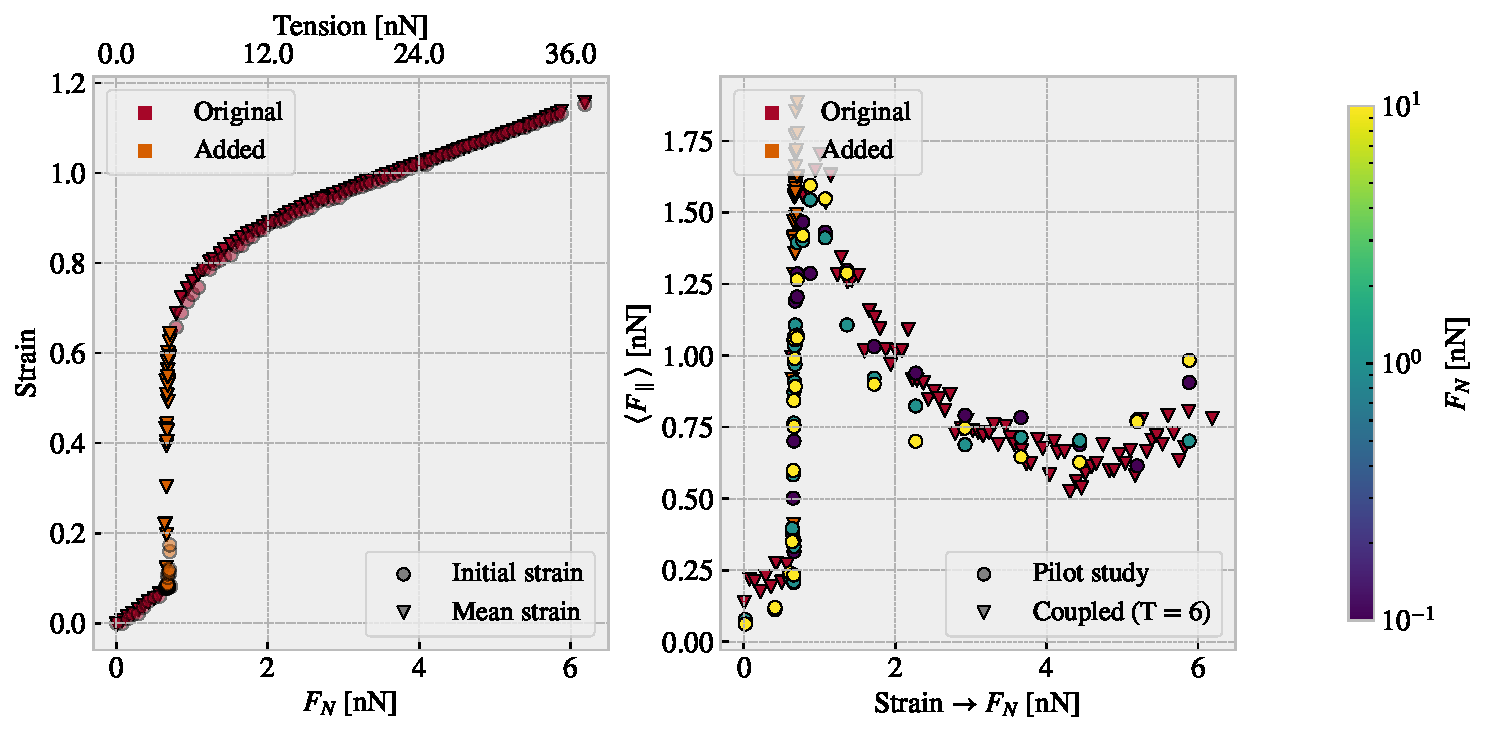
\includegraphics[width=\textwidth]{figures/negative_coefficient/manual_coupling_tension_hon2215.pdf}
    \caption{Honeycomb $(2,2,1,5)$}
    % \label{fig:}
  \end{subfigure}
  \hfill
  \caption{Evaluation of the friction response for a coupled system using (a) the Tetrahedron $(7,5,1)$ and (b) Honeycomb $(2,2,1,5)$ pattern.  The pull blocks are allowed to move relative to each other under the influence of a tension force $F_t$ modeled as $F_t = RF_N$ for normal load $F_N$ and a ratio $R=6$. The right panel shows the friction vs.\ stretch curve in comparison to the locked pull block system and constantly defined normal from the pilot study (\cref{fig:multi_stretch}). The left panel shows the strain-tension curve. For the Honeycomb pattern, we added more data points in the region where the strain-tension curve changed rapidly.}
  \label{fig:negfric}
\end{figure}

Generally, we observe from \cref{fig:negfric} that the data points of the
coupled system aligns reasonable well with the mapped data points from the pilot
study. This indicates that the simultaneous loading and straining of the system
does not suppress the underlying mechanism governing the non-linear trends. For
the Tetrahedron pattern we find an almost linear strain-tension curve which
makes for a recognizable trend in the friction-load curve similar to that seen
in the friction-strain curve in~\cref{fig:multi_stretch}. In both cases, we
also notice that the initial and the mean strains aligns rather well. This
suggest that the sliding does not contribute to a significantly increased
tension in the sheet which would otherwise lead to an increased strain as well.
For the Honeycomb pattern, we find an interesting trend for the strain-tension
curve. At low tension, the curve of the strain is increasing seemingly linearly
with strain, but a drastic increase in strain happens at a tension of \SI{4.5}{nN} ($F_N = \SI{0.75}{nN}$) transitioning from a strain of roughly 0.08 to 0.7. Eventually
this settles off into a linear trend before reaching the rupture point. This
reflects the reason for decreasing the loading speed and adding more data points
to fill this gap in strain-tension curve. The rapid increase in the strain-load
curve makes for a similar rapid increase in the friction-load curve as well.
Hence we find that the Honeycomb coupled system essentially exhibit an intial discontinuous increase in friction with load, which is then followed by a longer region of  decreasing friction with load. When considering the simulation frames in
\cref{sec:sheet_stretch} we notice that the strain range covered in this transition aligns rather well with the unfolding of the honeycomb pattern. We
have previously noted that the Honeycomb pattern unfolds in segments buckling
one at a time. We observe that this unfolding is initiziated after passing a minimum tension. During the unfolding phase the friction increases, but immediately after friction decrease with further straining. Once again, this highligts that this transition might of interest for further investigations in order to get a better understanding of the underlying mechanisms being in play.

From the results in~\cref{fig:negfric} we have found that our proposed coupled
system, based on a $T = 6$ tension-load coupling, demonstrates a significant
negative friction coefficient in certain load regions. By considering the
maximum and minimum friction points along the friction-strain curve we find that
this correponds to minimal friction coefficients $\mu_{\min}$ on the order of
\begin{align}
  &\text{Tetrahedron:} \quad \mu_{\min} \sim \frac{\SI{0.31}{nN} - \SI{0.90}{nN}}{\SI{6.55}{nN} - \SI{4.65}{nN}} = -0.31& 
  &\text{Honeycomb:} \quad \mu_{\min} \sim \frac{\SI{0.53}{nN} - \SI{1.88}{nN}}{\SI{4.31}{nN} - \SI{0.71}{nN}} = -0.38.&
  \label{eq:coupled_mu_estimate}
\end{align}
This result supports that the use of Kirigami sheet in a coupled system can be used to achieve a negative friction coefficients. In the pilot study (\cref{eq:pilot_study_mu_estimate}) we estimated the Tetrahedron pattern to exhibit a coeffient following $-R \SI{12.75}{nN}$ smaller than the Honeycomb following $-R \SI{2.72}{nN}$. From the results in~\cref{eq:coupled_mu_estimate} we find that the resulting coefficients a closer in value which we attribute to the difference in the strain-tension curve. However, we notice that both values can be scaled by increasing the strain-load coupling $T$, which would make for a more negative slope. 